\chapter{Background concepts}

\label{background}

\section{Explainable artificial intelligence}

In this section, we lay out background concepts for Explainable Artificial Intelligence (XAI) which have been largely adopted from \citet{arrieta2020explainable}. The study is particularly helpful for us since it summarizes the findings of approximately 400 XAI contributions and presents these findings in the form of well-defined concepts and taxonomies. In addition, the study discusses future directions of XAI research. We start off by providing definitions from the study, along with accompanying remarks taken either directly from the study or paraphrased for brevity.

\subsection{Transparency}

\begin{definition}[Transparency]
  A model is considered to be transparent if by itself it is understandable. Since a model can feature different degrees of understandability, transparent models are divided into three categories: simulatable models, decomposable models and algorithmically transparent models. 
\end{definition}

\begin{remark}
  \textit{Simulatability} denotes the ability of a model of being simulated or thought about strictly by a human, hence complexity takes a dominant place in this class.
\end{remark}

\begin{remark}
  \textit{Decomposability} stands for the ability to explain each of the parts of a model (input, parameter and calculation).
\end{remark}

\begin{remark}
  \textit{Algorithmic transparency} deals with the ability of the user to understand the process followed by the model to produce any given output from its input data.
\end{remark}

\begin{remark}
  A model is considered transparent if it falls into one or more of the aforementioned transparency categories.
\end{remark}

\begin{remark}
  If a model cannot satisfy the requirements of being transparent, then it is classified as a \textit{black-box} model. 
\end{remark}

Examples of well-known transparent Machine Learning (ML) models are linear/logistic regressors, decision trees and rules-based learners. Similarly, common examples of non-transparent or black-box ML models are tree ensembles and deep neural networks. \citet{arrieta2020explainable} provide extensive justifications using the aforementioned three criteria in conducting model classifications into the transparent and black-box categories. We would direct the reader to their study for a full analysis and justification of these classifications.

\subsection{Explainability and XAI}

\begin{definition}[Explainability]
  Explainability is associated with the notion of explanation as an interface between humans and a decision maker that is, at the same time, both an accurate proxy of the decision maker and comprehensible to humans. 
\end{definition}

\begin{definition}[Explainable Artificial Intelligence]
  Given an audience, an \textbf{explainable} Artificial Intelligence is one that produces details or reasons to make its functioning clear or easy to understand.
\end{definition}

\citet{arrieta2020explainable} observe that black-box ML models are increasingly being employed to make important predictions in critical contexts, citing high-risk areas such as precision medicine and autonomous vehicles. Of particular relevance to the field of Natural Language Processing (NLP), the study notes a myriad of issues related to inductive biases within training data sets and the ethical issues involved with using black-box models trained on such data sets. As a result, they describe the increased demand for transparency in black-box ML models from the various stakeholders in Artificial Intelligence (AI). In addition, \citet{arrieta2020explainable} concretize the presence of a target audience for XAI; implying that different XAI techniques should be employed for different target audiences. In their study, they provide examples of target audiences such as domain experts, end-users and managers (Figure \ref{fig:xai_target_audience}).

\begin{figure}[t]
  \centering
  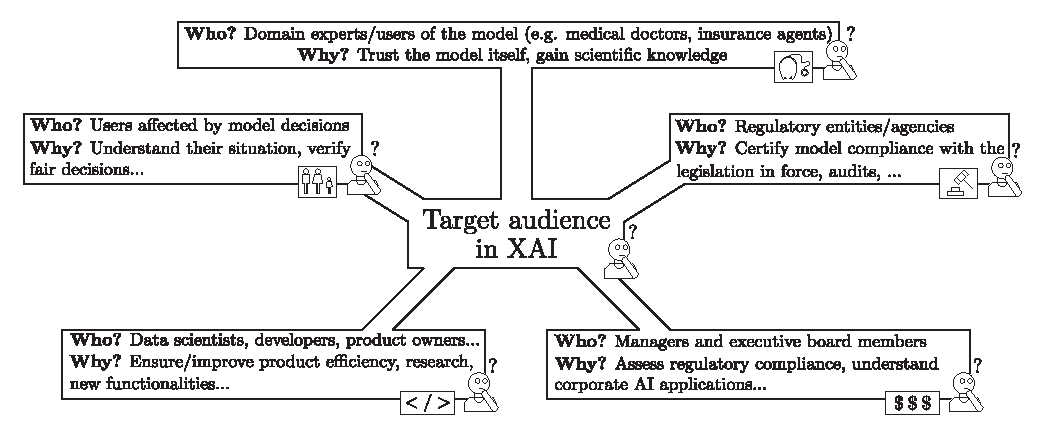
\includegraphics[trim={0.1cm 0.1cm 0.1cm 0.1cm},clip,width=14cm]{pdfs/xai_target_audience}
  \caption{Examples of various target audiences in XAI \citep{arrieta2020explainable}}
  \label{fig:xai_target_audience}
\end{figure}

\subsection{Explainability techniques}

Based on the aforementioned classification of ML models into transparent and black-box models, \citet{arrieta2020explainable} expound on explainability techniques for each of these model types. Due to their transparent nature, the study states that transparent ML models are usually explainable in themselves to most target audiences and therefore usually do not require any external technique to extract explanations. The study does however highlight some target audiences, such as non-expert users, who may require external explainability techniques such as model output visualizations in order to explain the inner workings of transparent ML models.

For the case of non-transparent or black-box models, \citet{arrieta2020explainable} argue that separate or external techniques must be utilized in order to reasonably explain these models. Such explainability techniques are referred to in the study as post-hoc explainability techniques; which is derived from the idea that explanations for such models are usually extracted after the modelling procedure. Notable examples of post-hoc explainability techniques include local explanations, feature relevance and explanations by simplification. Below we provide definitions for these methods, which have been adapted from \citet{arrieta2020explainable}:

\begin{definition}[Local explanations]
  Local explanations tackle explainability by segmenting the solution space and giving explanations to less complex solution subspaces that are relevant for the whole model.
\end{definition}

\begin{remark}
  Two well-known examples of local explainability techniques are Local Interpretable Model-Agnostic Explanations (LIME; \citealt{lime}) and G-REX \citep{konig2008g}.
\end{remark}

\begin{definition}[Feature relevance]
  Feature relevance explanation methods clarify the inner functioning of a model by computing a relevance score for its managed variables. These scores quantify the affection (sensitivity) a feature has upon the output of the model.
\end{definition}

\begin{remark}
  A well-known feature relevance explainability technique is known as the Shapley Additive Explanations (SHAP; \citealt{lundberg2017unified}). Another similar feature relevance explainability technique is known as the occlusion sensitivity method \citep{zeiler2014visualizing}.
\end{remark}

\begin{definition}[Explanations by simplification]
  Explanations by simplification collectively denote those techniques in which a whole new system is rebuilt based on the trained model to be explained. This new, simplified model usually attempts at optimizing its resemblance to its antecedent functioning, while reducing its complexity, and keeping a similar performance score.
\end{definition}

\begin{remark}
  We hereby refer to the original black-box model as an \textit{oracle} model and the simplified version of the model as the \textit{proxy} model. Furthermore, we qualify that all proxy models must be able to globally approximate their respective oracle models. This is in constrast to local explanations which only approximate subsets of oracle models.
\end{remark}

\begin{remark}
  \citet{bastani2017interpretability} and \citet{tan2018distill} are examples of studies that extract and distill simpler proxy models from complex oracle models.
\end{remark}

Through a survey of recent literature on explanations by simplification applied in the Natural Language Processing (NLP) field, we came across several prominent studies employing explanations by simplification to simplify black-box neural networks into constituent Finite-State Automata (FSA) and/or Weighted Finite-State Automata (WFSA) \citep{schwartz2018sopa,peng2018rational,DBLP:journals/corr/abs-1905-08701,wang2019state,jiang2020cold}. We expound more on WFSA and \citet{schwartz2018sopa} in Sections \ref{wfsa} and \ref{sopa} respectively.

\subsection{Key insights}

\section{Straight-through estimator}

\section{Weighted finite-state automata}

\label{wfsa}

\begin{definition}[Semiring; \citealt{kuich1986linear}]
  A semiring is a set $\mathbb{K}$ along with two binary associative operations $\oplus$ (addition) and $\otimes$ (multiplication) and two identity elements: $\bar{0}$ for addition and $\bar{1}$ for multiplication. Semirings require that addition is commutative, multiplication distributes over addition, and that multiplication by $\bar{0}$ annihilates, i.e., $\bar{0} \otimes a = a \otimes \bar{0} = \bar{0}$.

\begin{remark}
  Semirings follow the following generic notation: $\langle \mathbb{K}, \oplus, \otimes, \bar{0}, \bar{1} \rangle$.
\end{remark}

\begin{remark}
  A simple and common semiring is the real or sum-product semiring: $\langle \mathbb{R}, +, \times, 0, 1 \rangle$. Two important semirings for this thesis are shown below.
\end{remark}

\begin{remark}
  \textbf{Max-sum} semiring: $\langle \mathbb{R} \cup \{-\infty\}, \text{max}, +, -\infty, 0 \rangle$
\end{remark}

\begin{remark}
  \textbf{Max-product} semiring: $\langle \mathbb{R}_{>0} \cup \{-\infty\}, \text{max}, \times, -\infty, 1 \rangle$
\end{remark}

\end{definition}

\begin{definition}[Weighted finite-state automaton; \citealt{peng2018rational}]
  A weighted finite-state automaton over a semiring $\mathbb{K}$ is a 5-tuple $\mathcal{A} = \langle \Sigma, \mathcal{Q}, \mathcal{T}, \lambda, \rho \rangle$, with:

  \begin{itemize}
    \itemsep0em 
    \item[--] a finite input alphabet $\Sigma$;
    \item[--] a finite state set $\mathcal{Q}$;
    \item[--] transition weights $\mathcal{T}: \mathcal{Q} \times \mathcal{Q} \times (\Sigma \cup \{\epsilon\}) \rightarrow \mathbb{K}$;
    \item[--] initial weights $\lambda: \mathcal{Q} \rightarrow \mathbb{K}$; 
    \item[--] and final weights $\rho: \mathcal{Q} \rightarrow \mathbb{K}$.
  \end{itemize}

  \begin{remark}
    $\epsilon \notin \Sigma$ refers to special $\epsilon$-transitions that may be taken without consuming any input.
  \end{remark}

  \begin{remark}
    Self-loop transitions in $\mathcal{A}$ refer to special transitions which consume an input while staying at the same state.
  \end{remark}
  
  \begin{remark}
    $\Sigma^{*}$ refers to the (possibly infinite) set of all strings over the alphabet $\Sigma$.
  \end{remark}
   
\end{definition}

\begin{definition}[Path score; \citealt{peng2018rational}]

  Let $\pmb{\pi} = \langle \pi_1, \pi_2, \dots, \pi_n \rangle$ be a sequence of adjacent transitions in $\mathcal{A}$, with each $\pi_i = \langle q_i, q_{i+1}, z_i \rangle \in \mathcal{Q} \times \mathcal{Q} \times (\Sigma \cup \{\epsilon\})$. The path $\pmb{\pi}$ derives the $\epsilon$-free string $\pmb{x} = \langle x_1, x_2, \dots, x_m \rangle \in \Sigma^{*}$; which is a substring of the $\epsilon$-containing string $\pmb{z} = \langle z_1, z_2, \dots, z_n \rangle \in (\Sigma \cup \{\epsilon\})^{*}$. $\pmb{\pi}$'s score in $\mathcal{A}$ is given by:
  
\end{definition}

\begin{equation}
  \mathcal{A}[\pmb{\pi}] = \lambda(q_1) \otimes \Bigg( \bigotimes_{i=1}^n \mathcal{T}(\pi_i) \Bigg) \otimes \rho(q_{n+1})
\end{equation}

\begin{definition}[String score; \citealt{peng2018rational}]

Let $\Pi(\pmb{x})$ denote the set of all paths in $\mathcal{A}$ that derive $\pmb{x}$. Then the string score assigned by $\mathcal{A}$ to string $\pmb{x}$ is given by:
  
\end{definition}

\begin{equation}
  \mathcal{A}[\![\pmb{x}]\!] = \bigoplus_{\pmb{\pi} \in \Pi(\pmb{x})} \mathcal{A}[\pmb{\pi}]
\end{equation}

\begin{remark}
  Since $\mathbb{K}$ is a semiring, $\mathcal{A}[\![\pmb{x}]\!]$ can be efficiently computed using the Forward algorithm \citep{baum1966statistical}. Its dynamic program is summarized below without $\epsilon$-transitions for simplicity. $\Omega_i(q)$ gives the aggregate score of all paths that derive the substring $\langle x_1, x_2, \dots, x_i \rangle$ and end in state $q$:
 
\begin{subequations}
  \begin{align}
    \Omega_0(q) &= \lambda(q) \\
    \Omega_{i+1}(q) &= \bigoplus_{q' \in \mathcal{Q}} \Omega_i(q') \otimes \mathcal{T}(q',q,x_i)  \\
    \mathcal{A}[\![\pmb{x}]\!] &= \bigoplus_{q \in \mathcal{Q}} \Omega_n(q) \otimes \rho(q)
  \end{align}
\end{subequations}

\end{remark}

\begin{remark}
  The Forward algorithm can be generalized to any semiring \citep{eisner2002parameter} and has a runtime of $O(|Q|^3 + |Q|^2|\pmb{x}|)$ \citep{schwartz2018sopa}; notably with a linear runtime with respect to the length of the input string $\pmb{x}$.
\end{remark}

\begin{remark}
  A special case of Forward is the Viterbi algorithm, where the addition $\oplus$ operator is contrained to the maximum function \citep{viterbi1967error}. Viterbi therefore returns the highest scoring path $\pmb{\pi}$ that derives the input string $\pmb{x}$.
\end{remark}

\section{Soft patterns}
\label{sopa}

%%% Local Variables: 
%%% mode: latex
%%% TeX-master: "main"
%%% End: 
